\chapter{3 Component}
The three components of Machine learning are \textbf{model,data and loss}, all is a combination of this 3 components in different way.

\section{Data}
Data are a set or a collection of data point and the data points could be objects, records, cases, samples, entities, or instances that carries information called feature or label.
Features are low-level properties easy to measure or compute instead labels are high level quantity of interest difficult to measure or determine. They need to be in good number because we should use only most relevant features but not fewer, and missing some relevant feature is really bad for accuracy. Also use irrelevant features waste computational power and might cause overfitting.

Label is \textbf{design choice} because you choose the label of a data point, by choosing label you define the ML problem or learning task. The labels could be categorical or numerical, for the first we can choose also between Binary or multi class classification instead for the numerical we have a regression task
\begin{figure}[H]
    \centering
    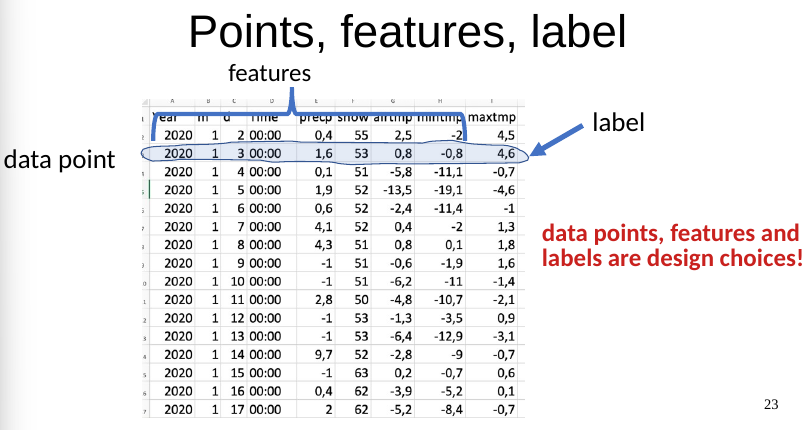
\includegraphics[scale=0.4]{images/3Comp/3Comp1.png}
    \caption{Example of tabular Data}
    \label{fig:enter-label}
\end{figure}
The feature can be seen as a matrix: \\
$ X = (x^{(1)} , x^{(2)}, \dots , x_{(m)})^t = \begin{bmatrix}
    x_1^{(1)} & x_2^{(1)} & \dots & x_n^{(1)} \\
    x_1^{(2)} & x_2^{(2)} & \dots & x_n^{(2)} \\
    \vdots & \vdots & \ddots & \vdots \\
    x_1^{(m)} & x_2^{(m)}& \dots &x_n^{(m)}
\end{bmatrix}
$\\
The labels as $y = (y_1, y_2,\dots, y_3 ) \in \mathbb{R}^{mxn}$\\
The data are the sum of them $D = {(x^{(1)} , y^{(1)}), \dots , (x^{(m)} , y^{(m)})}$.

\section{Model}
Model is another important part of Machine learning since we have to learn an hypothesis $ h \in H$ such that $h(x)\approx y$ \quad $h: X \rightarrow Y $, every model has several hypothesis but we have to choose the one that have the right number because a larger model can contain good hypothesis but maybe can overfitting, instead smaller are easier to fit computational resources, but they can not represent the real data or be too simple.
We can have different model due to the nature of the function we want to use linear, polynomial, decision tree or Artificial neural network to design our model.
\begin{figure}[H]
\centering
    \begin{subfigure}{.4\textwidth}
        \centering
        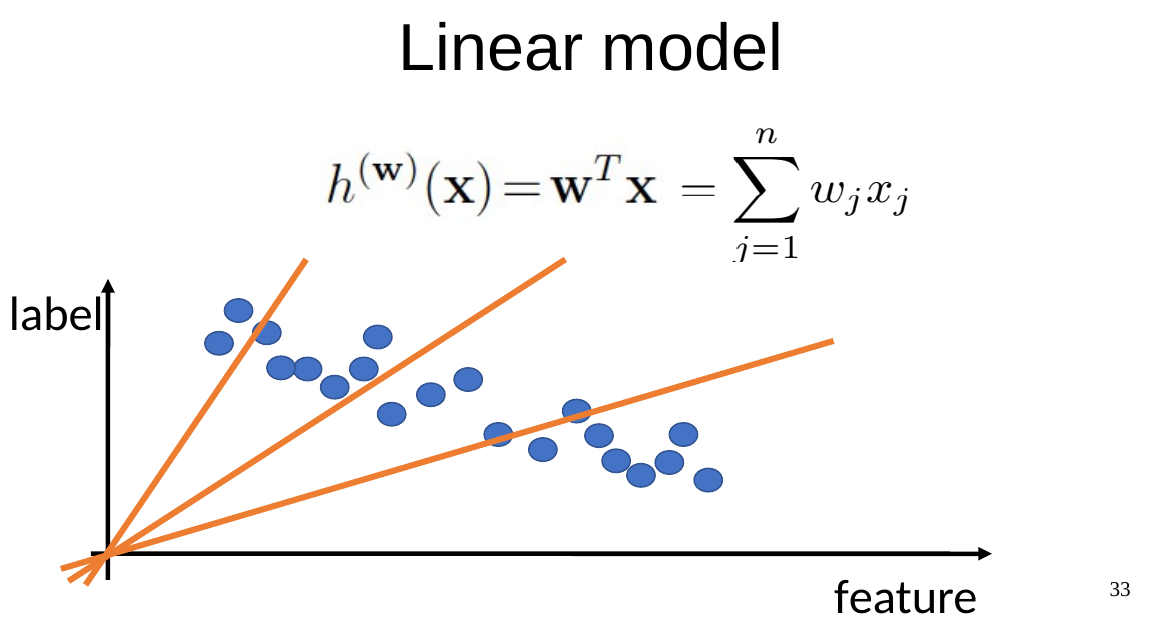
\includegraphics[width=1\linewidth]{images/3Comp/3comp2.png}
        \caption{}
        \label{fig:sub1}
    \end{subfigure}
    \begin{subfigure}{.4 \textwidth}
        \centering
        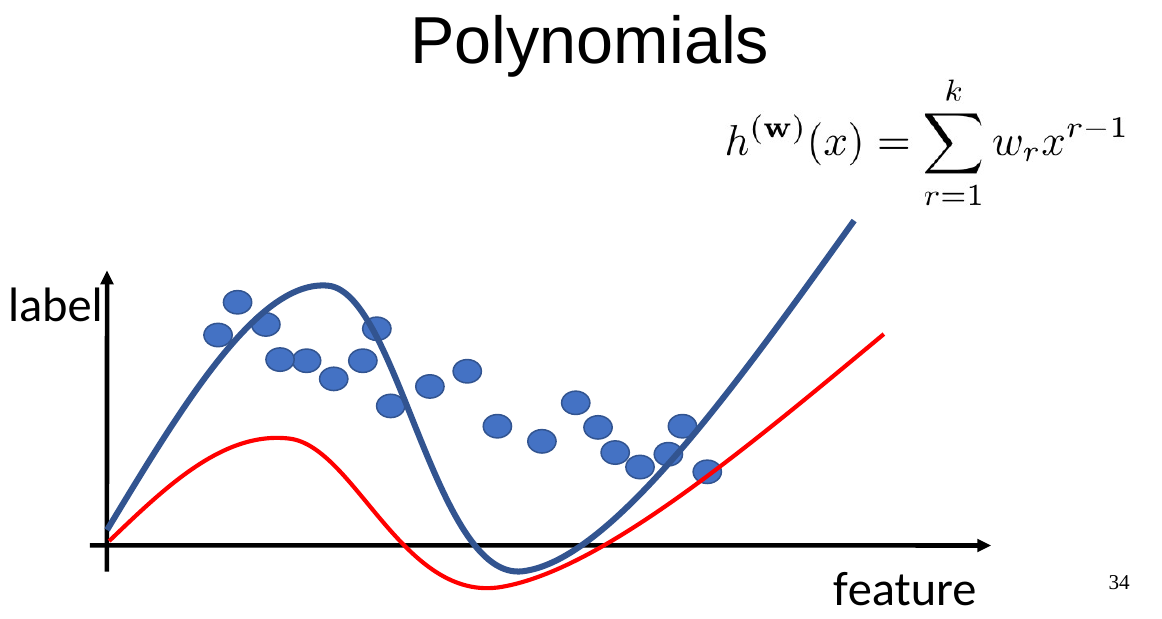
\includegraphics[width=1\linewidth]{images/3Comp/3comp3.png}
        \caption{}
        \label{fig:sub1}
    \end{subfigure}
    \caption{}
\end{figure}
\begin{figure}[H]
\centering
    \begin{subfigure}{.4\textwidth}
        \centering
        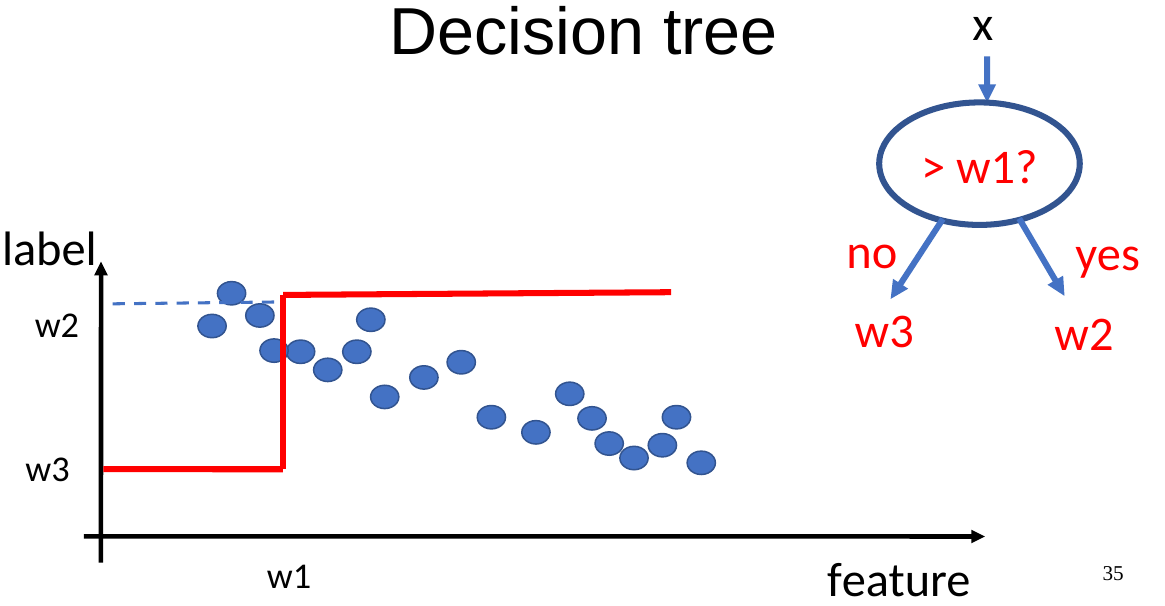
\includegraphics[width=1\linewidth]{images/3Comp/3comp4.png}
        \caption{}
        \label{fig:sub1}
    \end{subfigure}
    \begin{subfigure}{.4 \textwidth}
        \centering
        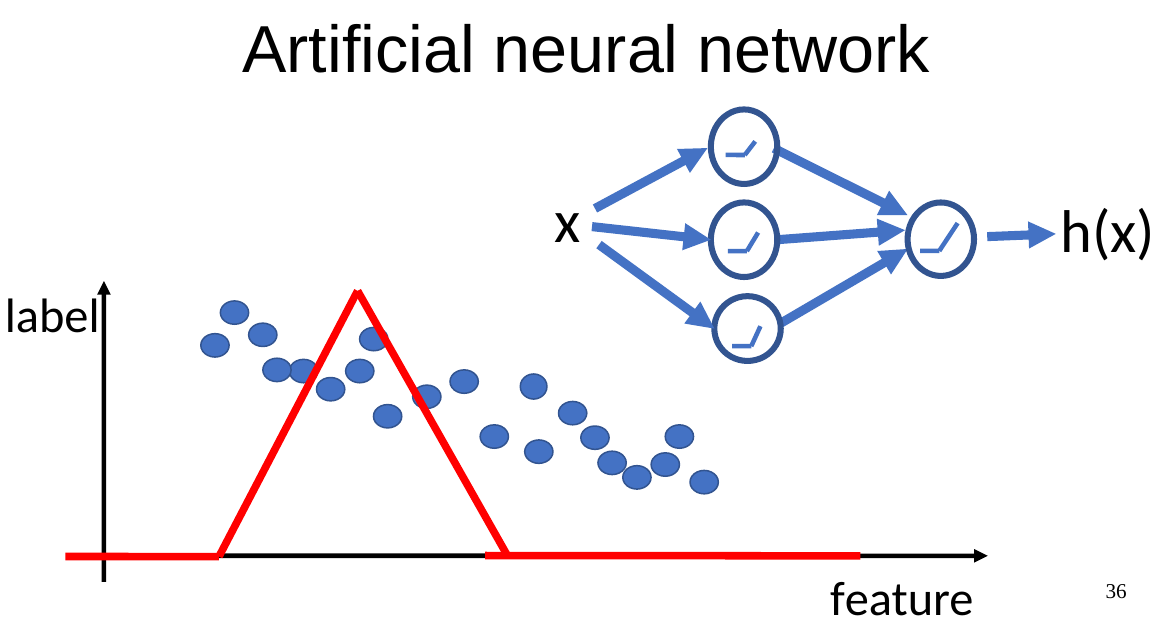
\includegraphics[width=1\linewidth]{images/3Comp/3comp5.png}
        \caption{}
        \label{fig:sub1}
    \end{subfigure}
    \caption{}
\end{figure}
To choose a model we have to consider and weigh 3 factors: \textbf{interpretability}, \textbf{computational} \textbf{complexity} and statistical accuracy, in fact the hypothesis has to be \textbf{sufficiently small} that means has much small as we can to have an optimal representation without overfit the model
\begin{figure}[H]
    \centering
    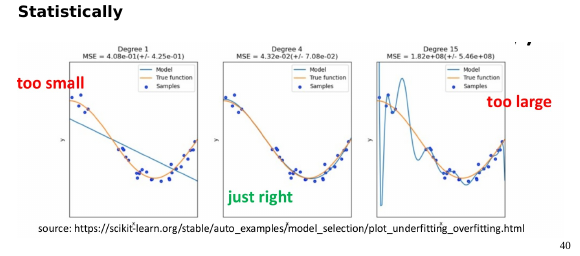
\includegraphics[scale=0.5]{images/3Comp/3comp6.png}
    \caption{Visual representation of sufficiently small}
    \label{fig:enter-label}
\end{figure}

\section{Loss}
The loss (funzione di costo in italiano) is the quantitative measure of prediction error obtained when using hypothesis h to predict label y’ of datapoint with features x’, there are different measure like the squared error loss $ L:= (\overline{y} - y)^2$ or the absolute error loss $L:= |\overline{y}-y|$. The binary classification is a different type which can have only a loss equal to 0 if we are correct and 1 if we did a mistake. As the model, choosing a loss function is done by considering: statistical aspects (should favour “reasonable” hypothesis), computational aspects (must be able to minimize them) and Interpretation (what does log-loss = -3 mean ?)

In conclusion to be able to learn from data and predict a label from new features we have to choose the right model with the right loss function
\begin{figure}[H]
\centering
    \begin{subfigure}{.4\textwidth}
        \centering
        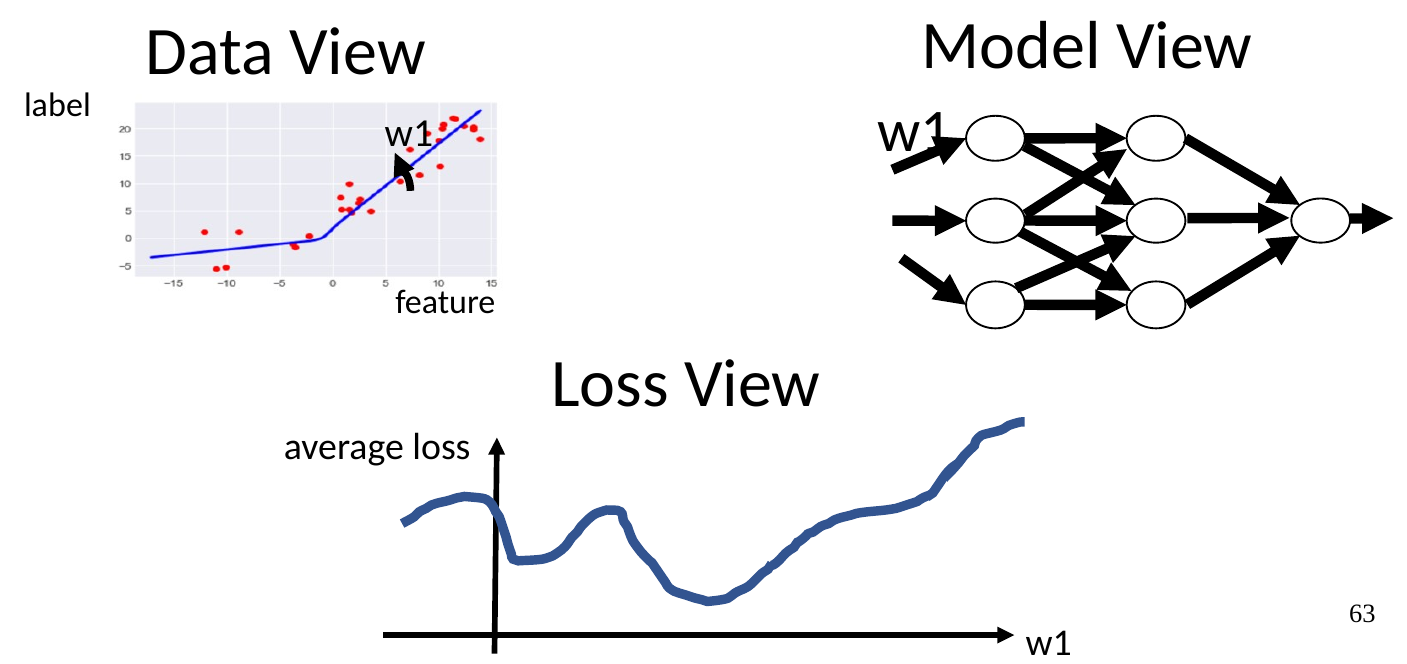
\includegraphics[width=1\linewidth]{images/3Comp/3comp7.png}
        \caption{Three views on machine learning}
        \label{fig:sub1}
    \end{subfigure}
    \begin{subfigure}{.4 \textwidth}
        \centering
        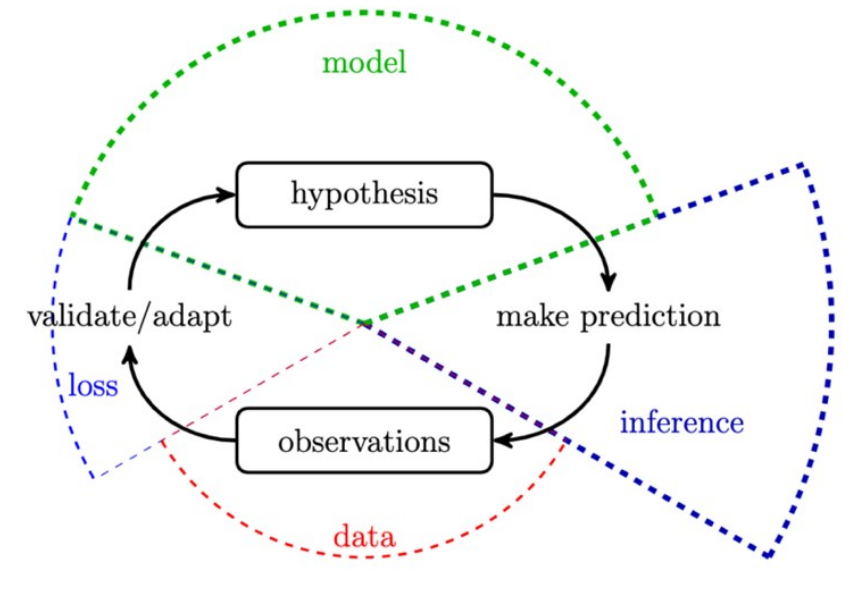
\includegraphics[width=1\linewidth]{images/3Comp/3comp8.png}
        \caption{ML process}
        \label{fig:sub1}
    \end{subfigure}
    \caption{}
\end{figure}

